\begin{figure}[tbp]
\centering
\begin{minipage}[t]{0.47\linewidth}
\centering
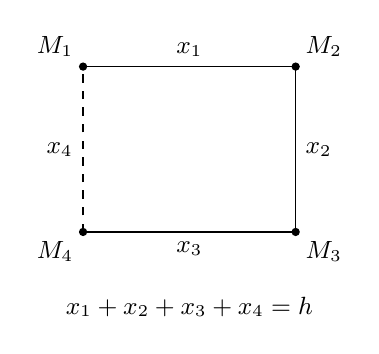
\begin{tikzpicture}[font=\small,line width=0.5pt]
 \coordinate (v1) at (0,0);
 \coordinate (v2) at (2.7,0);
 \coordinate (v3) at (2.7,-2.1);
 \coordinate (v4) at (0,-2.1);
 \draw (v1)--node[above]{$x_1$}(v2)
       --node[right]{$x_2$}(v3)
       --node[below]{$x_3$}(v4);
 \draw[dashed,thick] (v4)--node[left]{$x_4$}(v1);
 \foreach \v in {v1,v2,v3,v4} \fill (\v) circle (1.5pt);
 \node[above left] at (v1) {$M_1$};
 \node[above right] at (v2) {$M_2$};
 \node[below right] at (v3) {$M_3$};
 \node[below left] at (v4) {$M_4$};
 \node at (1.35,-3.05) {$x_1+x_2+x_3+x_4=h$};
\end{tikzpicture}
\end{minipage}\hfill
\begin{minipage}[t]{0.50\linewidth}
\centering
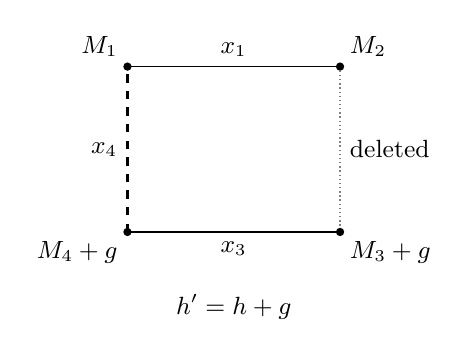
\begin{tikzpicture}[font=\small,line width=0.5pt]
 \coordinate (v1) at (0,0);
 \coordinate (v2) at (2.7,0);
 \coordinate (v3) at (2.7,-2.1);
 \coordinate (v4) at (0,-2.1);
 \draw (v1)--node[above]{$x_1$}(v2);
 \draw[densely dotted,gray] (v2)--node[right,text=black]{deleted}(v3);
 \draw (v3)--node[below]{$x_3$}(v4);
 \draw[dashed,thick] (v4)--node[left]{$x_4$}(v1);
 \foreach \v in {v1,v2,v3,v4} \fill (\v) circle (1.5pt);
 \node[above left] at (v1) {$M_1$};
 \node[above right] at (v2) {$M_2$};
 \node[below right] at (v3) {$M_3+g$};
 \node[below left] at (v4) {$M_4+g$};
 \node[align=center] at (1.35,-3.05)
   {$h'=h+g$};
\end{tikzpicture}
\end{minipage}
\caption{A site ring and the potential adjustment at one type and
one address, with $r=4$.  The dashed edge is the row-$4$ seam.
Left: every potential occurs twice in the sum, leaving $h$.
Right: after deleting row $2$, changing $h$ to $h+g$ and adding $g$
to $M_3,M_4$ preserves every retained readout.  The dotted segment
is absent from the retained corner graph.  The general proof uses
\Cref{offset:lem-gauge} on any nonwrapping component,
not only a cut site ring.}
\label{fig:projection-gauge}
\end{figure}
